% !Mode:: "TeX:UTF-8"
% !TEX root = tjumain.tex

\iffalse
\bibliography{reference/reference.bib} % 欺骗latextools获取bib文件
\fi

%%%%%%% 正文 %%%%%%%

\chapter{绪论}

\section{课题背景}

语言是人类交流沟通的重要方式,人们的绝大部分知识也是以语言文字的形式记载和流传下来的,它在人类的社会生活中起着至关重要的作用。随着时代的发展,计算机越来越广泛地渗透到人类社会的各个领域,语言文字信息也逐渐数字化,互联网技术的迅猛发展,人们摆脱了信息贫乏的桎梏,进入了一个信息极度丰富的社会。

在英剧《黑镜(Black Error)》中有一集是刻画女主人公在男友艾仕车祸去世后,在朋友的推荐下,利用艾仕在社交网络上留下的信息塑造了一个可以“完美”模仿艾仕的人工智能系统,可以和女主角语音交流。这个人工智能系统就是通过阅读艾仕的邮件、聊天记录等海量信息来了解他。理解语言这项人类的基本技能,也成为了众多科幻作品中人工智能的入门标配。在计算机学科和人工智能学科中,研究如何让机器理解语言已经成为了一个专门的研究领域,即自然语言处理。人工智能取得了一系列进展,并在各个领域取得了广泛应用,不过毋庸置疑的是,自然语言处理始终是实现自然人机交互愿望的一块重要技术基石。

自然语言处理的主要研究内容,是如何让计算机处理语言文字信息,以及实现人与计算机之间用自然语言进行有效沟通。然而,这是十分困难的,造成困难的根本原因是自然语言文本的各个层次上广泛存在的各种各样的歧义性,包括词语中的一词多义与多词同义、短语中多个词性所导致的语法歧义、句子中的语序不同却表达同样意义等等。解决这个问题可以抽象为判断两个文本是否匹配,比如:一个有歧义的文本表达的是一种含义,而另一个没有歧义的文本表达的也是同样的含义,若文本匹配系统判断两个文本匹配,则说明系统可以有效识别文本信息。

文本匹配是自然语言处理领域中的核心问题之一,目标是对于两个文本,给出它们,求出相似度,进而判断其是否匹配。许多任务,如问题复述、阅读理解、信息检索、机器翻译、自动文摘系统都可以归结成文本匹配问题。问题复述,即对相同语义的不同表达,可以抽象为判断两个句子的语义是否匹配;阅读理解,可以抽象为文章中信息和所问题目之间的匹配;信息检索,可以抽象为检索词和文档的匹配,机器翻译可以抽象为两种不同语言之间的匹配;自动文摘可以抽象为文章和摘要之间的匹配。

其中,以问题复述、信息检索、以及机器翻译为代表等多个任务,已经广泛应用在人们平时生活中的。问题复述可以应用在知乎、Quora等在线问答平台,用户可能会提问很多相似问题,判断两个问题是否表达了同样的语义,即两段文本是否匹配,十分重要。信息检索在生活中的应用,早已不止于人们耳熟能详的搜索引擎百度、谷歌,在微博、推特等社交媒体中,搜索已经作为独立的应用上线,微博搜索已经成为用户关注时事热点的主要来源,微信也提供了微信公众号文章搜索,历史记录搜索等,这些技术的关键都是文本匹配任务。因而文本匹配的研究具有重要的理论和应用价值。
\cite{zhang2010tree}。

\section{研究意义}
对于文本匹配问题的研究,可以应用在自然语言处理绝大部分任务中。根据使用场景的不同,可分为三类:短文本-短文本匹配,短文本-长文本匹配,长文本-长文本匹配。

\subsection{短文本-短文本匹配}
很长一段时间以来自然语言处理都在研究句子级的文本,即短文本。短文本和短文本的匹配在工业界应用最为广泛,如:问题复述、机器翻译、自动问答系统等。

以问题复述在机器学习中的经典方式为例,对于给定的两句话,首先要获得他们的单词表达,通过函数映射得到句子表达,然后将两个文本进行交互,提取它们的交互特征信息,最后综合前面一个或多个信息得到他们匹配程度的打分,这也是文本匹配任务的一般过程。问答系统,当前自动问答的大量工作主要是基于知识库进行检索,需要将问题和知识库中的候选答案进行匹配,返回按匹配程度从高到低排序序列。

机器翻译也很类似,如将一句话由语言A翻译成语言B,用在统计机器翻译中首先要从语言B的平行语料库中找到该句子的每个词语使用语言B的表示,这就需要用到单词级别的匹配技术。可以使用单词级别的词向量进行匹配。

\subsection{短文本-长文本匹配}
短文本和长文本的匹配在工业界也有许多应用,如信息检索、阅读理解、自动文摘等。

信息检索的主要过程是可以分为三部分:建立文档索引,查询召回候选文档,检索。首先要从预处理之后的文档集离线生成索引,用户输入查询语句,搜索引擎初步召回一批候选文档,将查询词或语句和候选文档进行文本匹配,将候选文档按匹配程度由高到低进行排序后返回。其中召回候选文档和检索是关键步骤,都需要用到文本匹配。召回候选文档时需要将生成的索引与用户查询进行匹配;检索则是通过计算查询语句和各个文档的语义相关度,得到他们之间的匹配程度,并进行排序后返回在网页上。召回候选文档和检索时由于候选文档相对较长,需要用到短文本与长文本的匹配。短文本与长文本的匹配方式与1.2.1中的整体方法类似,区别在于短文本得到句子表达即可,长文本表达的信息更多,还需要得到段落表达,而由于段落是以层次化的形式组织起来的,文本匹配时还需要考虑不同层次的匹配信息。

阅读理解的时候,要将阅读中的问题和原文章进行短文本-长文本匹配,而理解长文本语义与句子间的连贯、上下文、句子的歧义性有很大关联,因而采取什么样的形式表达长文本也是一个很大的难点。同时短文本和长文本的匹配存在着匹配的非对称性问题。

\subsection{长文本-长文本匹配}
长文本和长文本的匹配的应用,相对较少。原因是长文本组织层次丰富,同时存在上下文关联情况,因而长文本之间匹配的应用,如新闻推荐,往往可以先提取摘要,然后将摘要进行匹配。新闻推荐还可以使用主题模型,先得到两个文本的主题分布,再通过计算两个多项分布的距离,反映出他们之间的匹配程度。

\section{研究内容}

文本匹配的研究方式主要可分为传统方法,和机器学习方法。传统方法主要基于人工提取特征、设计规则,一个好的模型依赖于提取出的优质特征、规则,因而耗费人力较大,规则难以维护,系统也较为复杂。

近几年来,随着深度学习在语音识别、计算机视觉取得了突出进展,文本匹配也成为了当前深度学习研究的热点问题。基于深度学习的文本匹配模型,是利用深度神经网络,从文本中直接提取模式,并计算匹配程度得分。由于它可以直接从大量的数据中,端到端的学习特征,节省了人力物力。文本匹配的研究人员提出了许多深度学习模型,分别在不同的具体任务上有效。其中一个模型MatchSRNN在匹配任务结束后,通过回溯找到了两个句子的匹配路径,这符合人类在判断两个句子是否匹配的自然过程。但是使用传统方法,或者深度学习方法来找到匹配路径,需要大量特征、以及标注数据,来定义正确的匹配路径,成本和复杂度较高。因而本文希望找到一种可以生成匹配路径的方法。

最近,基于,在围棋领域战胜了人类高手李世石,引起了学术界的广泛关注。强化学习是机器学习的一个重要分支,一个完整的强化学习过程,可以让计算机由完全不了解任务,通过不断的尝试,从和环境的交互学习,最后找到规律,达到任务目的。强化学习算法本身就会和环境进行交互,从获得的奖励或惩罚中学习。这些奖或惩,其实就可以作为生成匹配路径的需要的大量数据,同时由于这种学习过程,强化学习在序列生成问题上表现突出,生成匹配路径本质是一种序列生成的过程,于是本文使用强化学习算法来模拟匹配路径的生成过程,从而计算匹配程度。

基于上述现状,本文使用强化学习方法来建模文本匹配问题,采用了马尔可夫决策过程(Markov Decision Process,MDP)方法本文的主要贡献如下:

针对文本匹配问题,设计了马尔可夫决策过程中的状态、动作、价值函数以及奖励函数,实现了基于价值迭算法(value iteration)的文本匹配模型,在在线问答平台 Quora 数据集训练模型,并进行优化,与经典的深度学习的文本匹配模型MatchPyramid 和 MatchSRNN 的结果进行比较,实验结果表明基于价值迭代算法的文本匹配模型,在各个评价准则下均优于其他经典文本匹配算法的效果。

\section{本文组织结构}
本文共分为六章,每章节的内容组织如下:

第一章为绪论部分,主要介绍了文本匹配任务的研究背景及意义,并说明了本文的主要贡献。首先由自然语言处理引出文本匹配这一重要任务,根据使用场景的不同分为三类,介绍了各自的经典任务以及实现方式,总结了当前文本匹配的研究现状,提出了基于强化学习的文本匹配模型。

第二章从两个方面介绍了国内外研究现状。第一方面是关于文本匹配的相关工作,主要介绍了模,从传统方法到深度到强化学习,另一方面是强化学习的研究现状,主要介绍了强化学习的基本概念、符号定义以及相关算法,为本文之后提出的模型打下基础。符号定义

第三章主要介绍文本匹配问题的详细描述,马尔可夫决策过程和面向文本匹配问题的马尔可夫决策过程
 符号定义与强化学习 符号定义 MDP

第四章介绍面向问奔跑(MDP方法) 价值迭代

第五章介绍(价值迭代)实验以及讨论

第六章对全文进行总结,展望未来的发展



\chapter{相关工作与国内外研究现状}

\section{文本匹配研究相关工作}
\label{sec:text_matching}
文本匹配是自然语言处理中的经典任务,早期文本匹配的研究大多是基 向量空间模型,如将文本从稀疏的高维空间映射到一个低维的向量空间的潜在语义分析模型\cite{Landauer1998AnIT}(Latent Semantic Analysis,LSA),主题模型\cite{Blei2003LatentDA}(Latent Dirichlet Allocation,LDA),然而这种利用统计推断发现数据潜在模式的方式在短文本上表现不好,也不能精准建模文本匹配中的语义相关程度。研究学者将机器翻译的思想引入文本匹配,Berger和Lafferty使用统计机器翻译模型计算文本间的匹配程度,将两个句子的匹配视为不同语言的翻译问题,实现了近义词之间的相互匹配映射。之后又有研究者从语义紧密度等度量出发来规避结构转义问题,从对网页打关键词标签来解决非对称匹配问题等,但这样人工提取特征的代价很大,无法挖掘隐含在大量数据中含义不明显的特征,同时还会导致逻辑非常复杂。

近年来,随着计算机计算能力的不断提升,互联网数据呈爆炸式增长,深度学习依靠利用大规模数据与高性能计算的优势在语音识别、计算机视觉均取得了突出进展,自然语言处理也成为了当前深度学习研究的热点领域。有不少研究学者们使用深度学习方法来解决文本匹配问题。

基于深度学习算法的文本匹配模型的过程大致如图所示~\ref{fig:deep_text_matching},首先将每个单词映射到词向量,利用函数得到短语或句子的中间表达,然后进行文本的交互形成匹配空间,再进一步提取其中的模式信息,最后综合前面所有信息得到匹配度得分。~\\
\begin{figure}[htbp!]
\centering
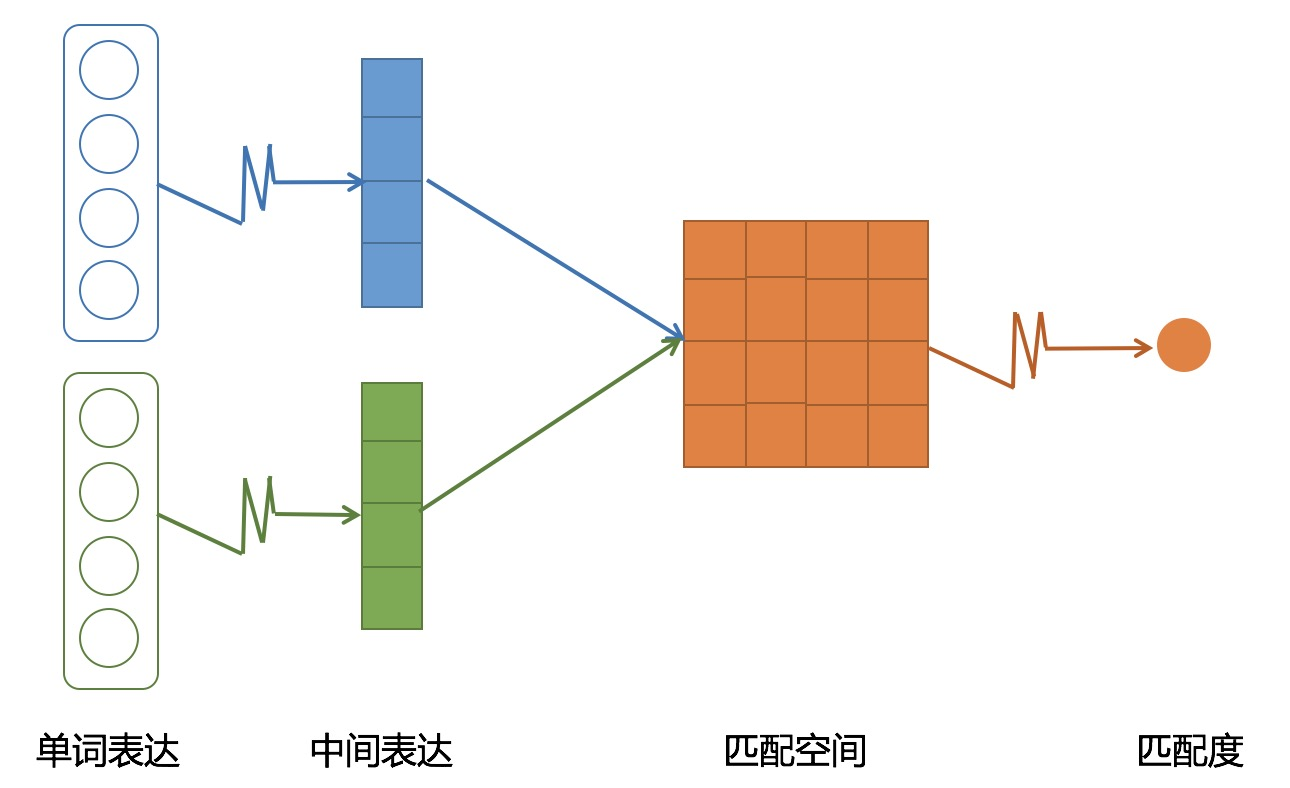
\includegraphics[width=0.75\textwidth]{figures/DeepTextMatching.jpg}
\caption{基于深度学习的文本匹配过程}\label{fig:deep_text_matching}
\vspace{-1em}
\end{figure}
~\\HUANG P S, et al.率先提出了深度语义结构模型\cite{Huang2013LearningDS}(Deep Structured Semantic Model, DSSM),这也是最早利用深度学习进行文本匹配的工作。主要针对查询和文档的匹配任务。它的数据是搜索引擎里查询与对应文档的点击日志,利用深度神经网络在一个连续的语义空间学习查询和文档的低维向量表示,通过余弦相似度计算两个文本的语义相似度。

深度语义结构模型如图\ref{fig:DSSM}主要分为3层:输入层、表示层、匹配层。输入层使用词哈希(Word Hashing)处理文文本,对于英文文本,将单词切分成三个字母为一组的单词。这样可以压缩空间,提高泛化能力。对于中文文本,以单字的一位有效编码(one-hot)进行输入。在表示层,采用词袋(Bag of words,BOW)的方式,输入一个4层深度神经网络\cite{hinton2006fast}(Deep Neural Network,DNN),输出128维的向量表示,匹配层利用cosine距离衡量两个语义向量的相似度,并使用softmax将查询与正样本的相似度转化为概率分布。

\begin{figure}[htbp!]
\vspace{1em}
\centering
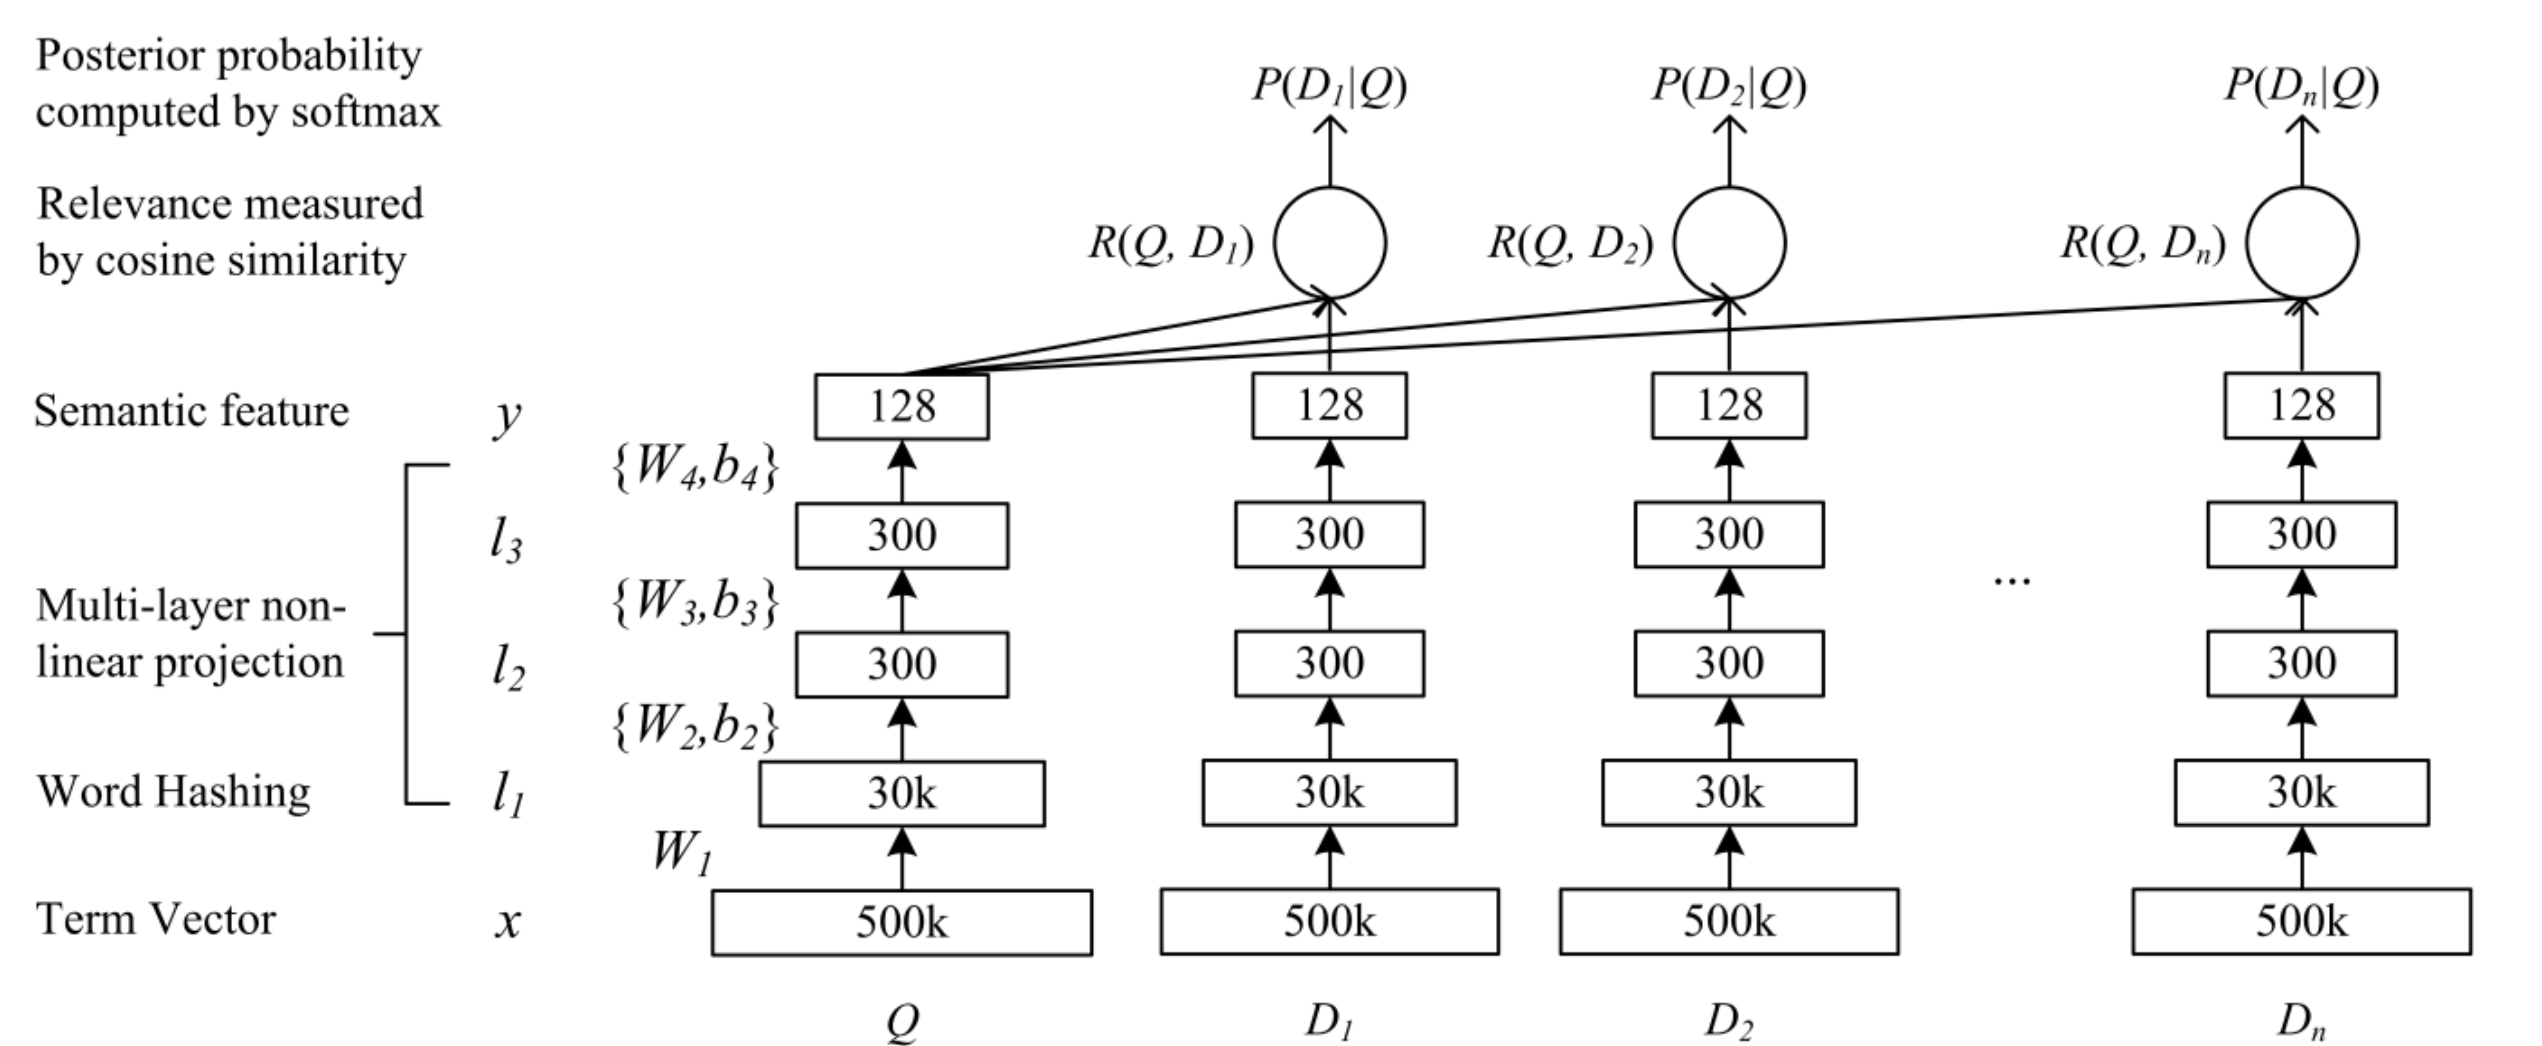
\includegraphics[width=1.0\textwidth]{figures/DSSM.png}
\caption{深度语义结构模型}\label{fig:DSSM}
\vspace{1em}
\end{figure}

这种方法可以减少对切词依赖,并提高对模型的泛化能力,因为语义可以服用,同时不同于Word2Vec和LDA的无监督学习,DSSM采用有监督学习方式,精准度较高。不过由于DSSM使用的全连接神经网络参数过多,难以训练,同时它采用词袋模型,缺失了语序信息和上下文信息。

针对DSSM的缺点,微软提出了使用卷积神经网络\cite{lecun1998gradient}(Convolutional Neural Network,CNN)提取上下文信息,即基于单词序列的卷积潜在语义模型\cite{Shen2014ALS}(Convolutional Latent Semantic Model,CLSM),与DSSM相比,CLSM主要对输入和表示层进行了改进,在输入层增加了单词滑动窗口(Word-n-gram),来提取序列信息。在表示层使用了卷积和池化结合的方式提取上下文信息。

\begin{figure}[htbp!]
\vspace{1em}
\centering
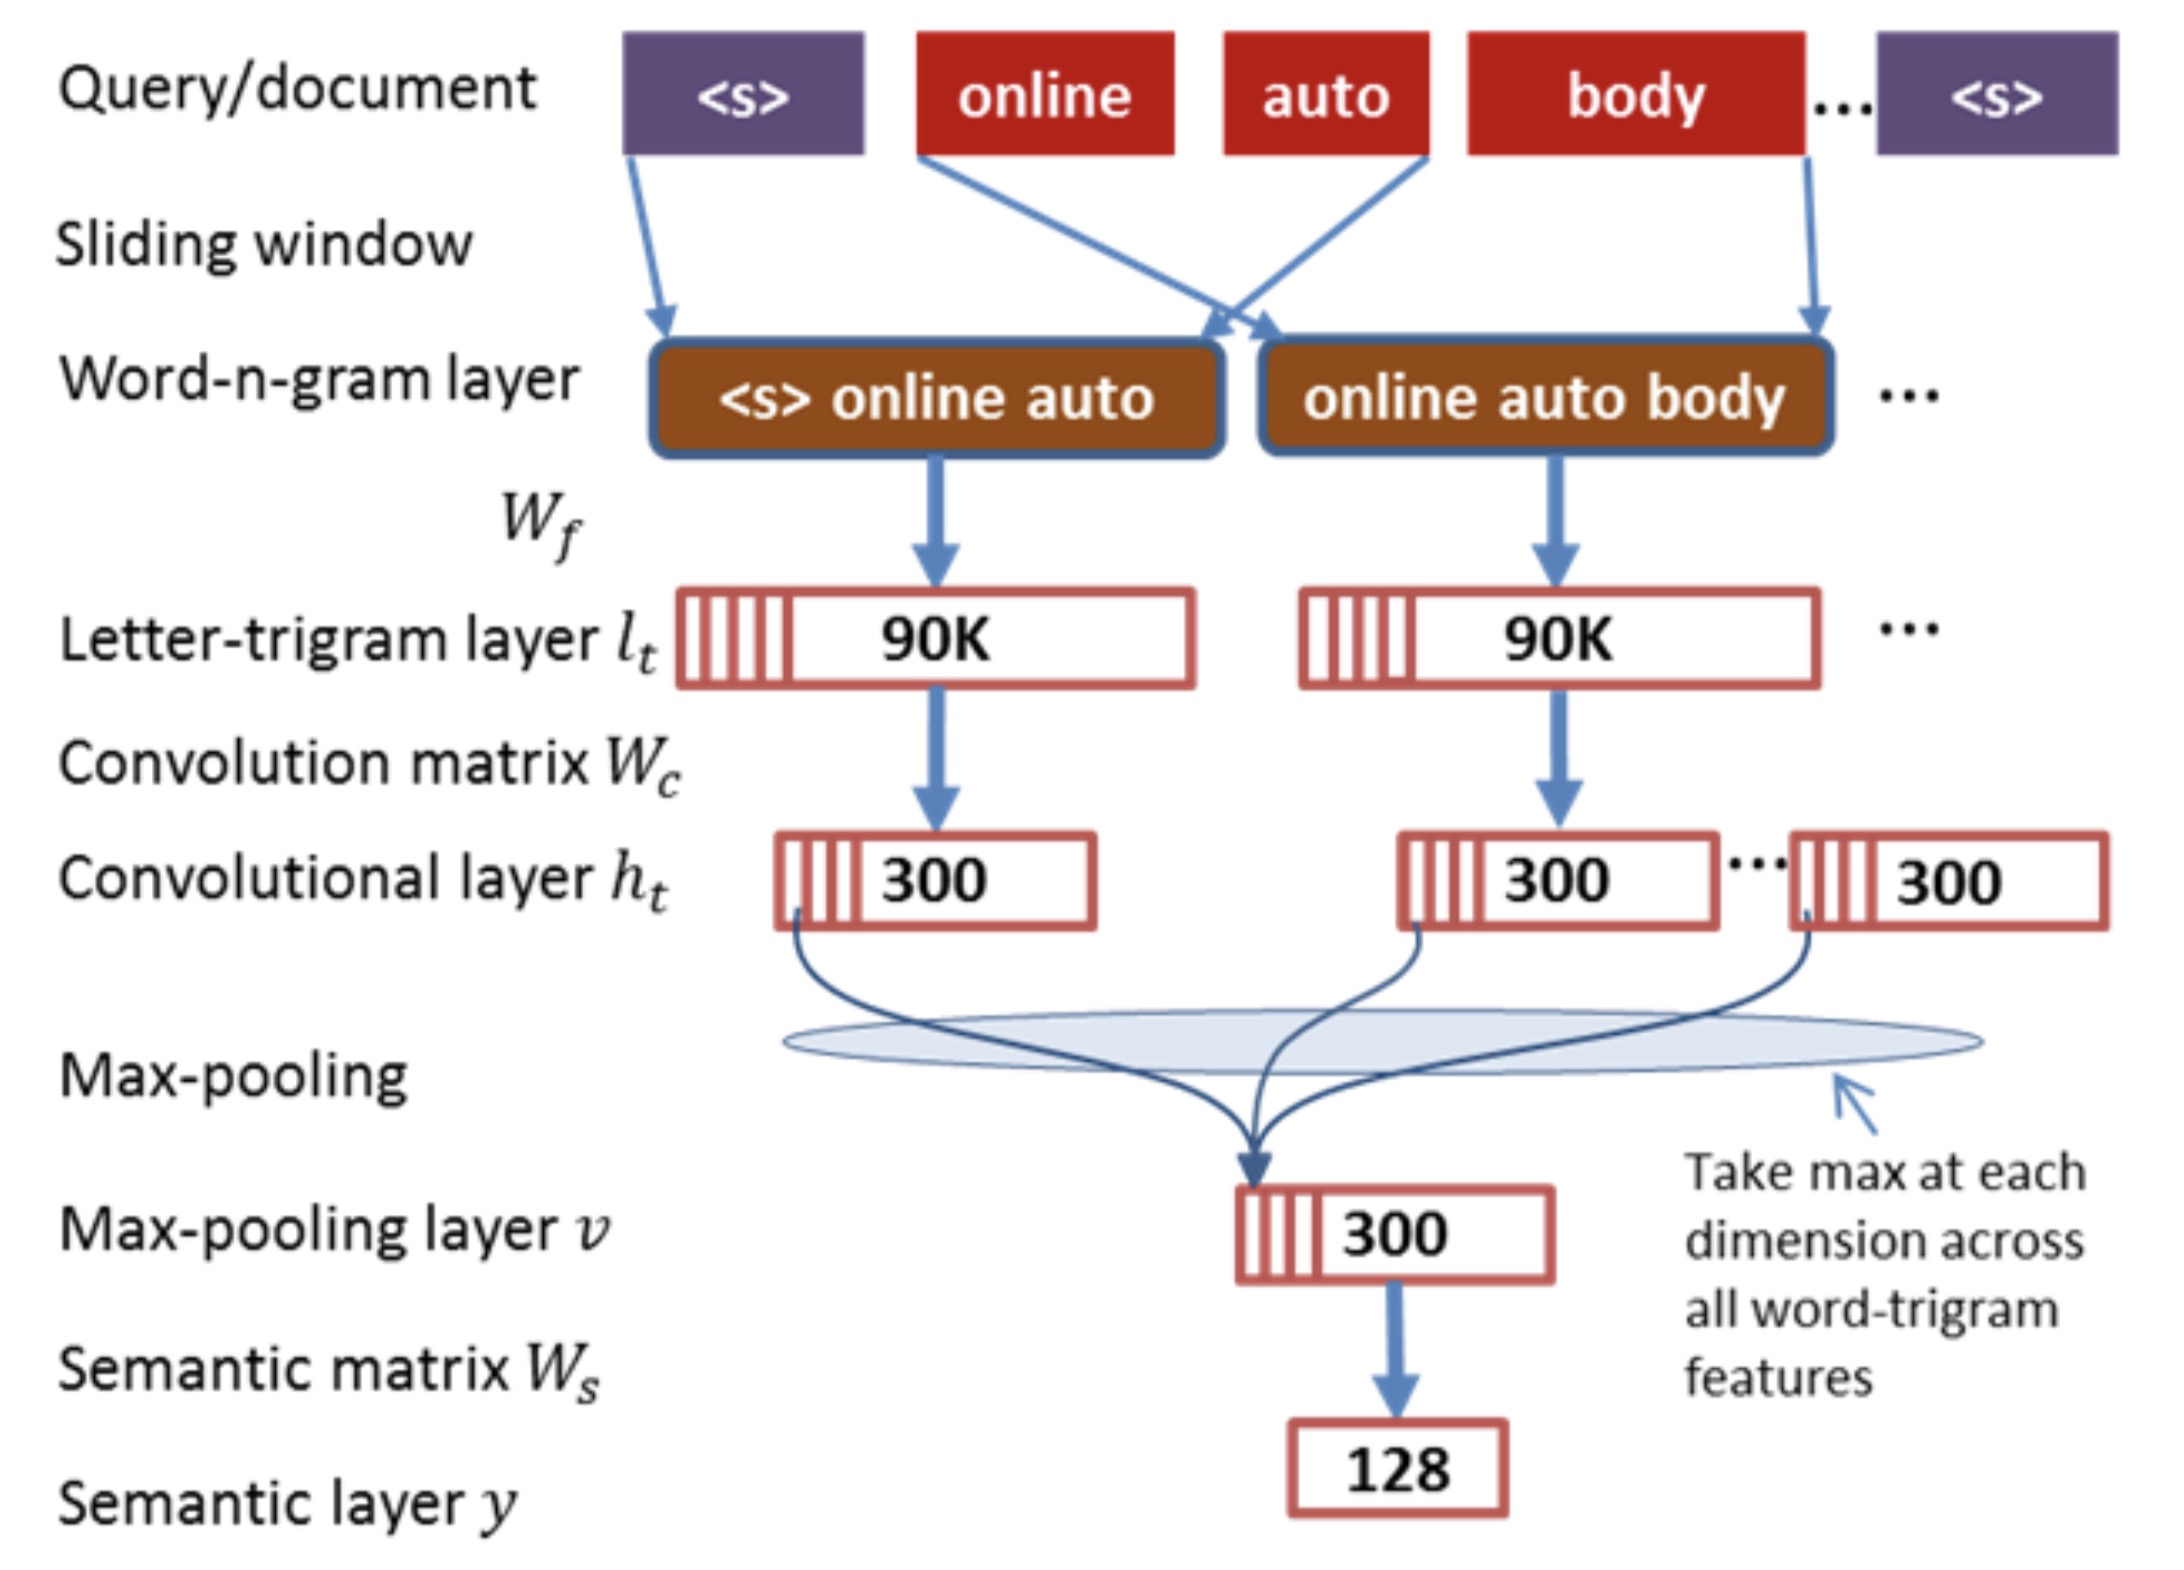
\includegraphics[width=0.75\textwidth]{figures/CLSM.jpg}
\caption{CLSM模型结构}\label{fig:CLSM}
\vspace{1em}
\end{figure}


图\ref{fig:CLSM},单词滑动窗口包含了上下文信息,对于滑动窗口内的词,类似DSSM,它将每个单词的3字母组合的词哈希向量连接得到最终的向量表示。在表示层包括了卷积层和池化层,卷积层中卷积核提取上下文特征。池化层使用最大化池化(Max-pooling)的方式为句子找到全局的上下文特征,最后利用全连接层将结果映射到一个128维的向量空间。匹配层和DSSM的相同,不做过多描述。

相比于DSSM,CLSM通过卷积和池化使得上下文信息得到较为有效的保留,但是由于卷积核大小的限制,对于间隔较远的上下文信息仍然难以捕捉。

针对上述问题,有人提出使用循环神经网络(Recurrent Neural Network,RNN)建模间隔较远的上下文信息。RNN可以被看做是同一神经单元的多次复制,各个神经单元共享参数,会把消息传递给下一个,这使得它可以很好的处理序列数据。图\ref{fig:RNN}描述了一个简单的RNN网络结构。

\begin{figure}[!htbp]
\vspace{1em}
\centering
  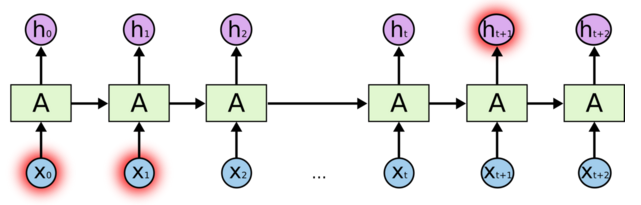
\includegraphics[width=0.8\textwidth]{figures/RNN.png}
  \caption{RNN 网络结构}
  \label{fig:RNN}       % Give a unique label
\vspace{1em}
\end{figure}


不过由于RNN的网络和序列长度有关,因此当RNN的序列长度过长时,梯度消失的情况会十分明显,导致RNN难以对长序列建模。为解决这个问题,有研究学者提出了长短时记忆网络LSTM\cite{Hochreiter1997LongSM},如图\ref{fig:LSTM}:
\begin{figure}[!htbp]
\vspace{1em}
\centering
  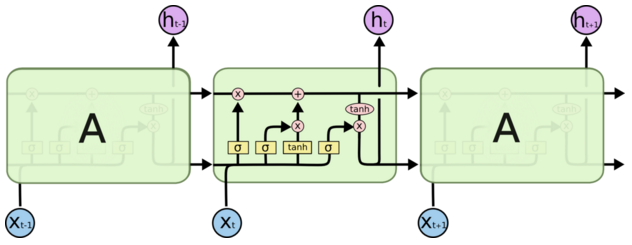
\includegraphics[width=0.8\linewidth]{figures/LSTM.png}
  \caption{LSTM 网络结构}
  \label{fig:LSTM}       % Give a unique label
\vspace{1em}
\end{figure}

LSTM可保留误差,用于沿时间和层进行反向传递。LSTM将误差保持在恒定的水平,让循环网络能够进行许多个时间步的学习(超过1000个时间步),从而打开了建立远距离因果联系的通道。由于本文提出的算法也用到了LSTM,接下来会重点介绍一下LSTM的工作原理。LSTM的关键就是细胞状态,它类似于传送带。直接在整个链上运行,只有一些少量的线性交互。信息在上面流传保持不变会很容易。LSTM 有通过“门”的结构来去除或者增加信息到细胞状态的能力。门是一种让信息选择式通过的方法,包含一个 sigmoid 神经网络层和一个pointwise乘法操作。

LSTM 利用忘记门(FORget gate)决定会从神经单元状态中丢弃的信息,利用输入门(input gate)确定被存放在细胞状态中的新信息,利用输出门(FORget gate)确定输出的信息:
\begin{equation}
\label{LSTM_eq}
\begin{aligned}
f_t&=\sigma(W_f[h_{t-1}, x_t] + b_f) \\
i_t&=\sigma(W_i[h_{t-1}, x_t] + b_i)\\
\tilde{C}_t &= \text{tanh}(W_C[h_{t-1}, x_t] + b_C)\\
o_t&=\sigma(W_o[h_{t-1}, x_t] + b_o)\\
h_t&=o_t\text{tanh}(\tilde{C}_t)
\end{aligned}
\end{equation}

LSTM通过这种方式,有效地避免了RNN网络的梯度消失问题。

LSTM-DSSM与CLSM的主要区别就是将CNN换成了LSTM。其整体网络结构如图\ref{fig:LSTM-DSSM}:

\begin{figure}[!htbp]
\vspace{1em}
\centering
  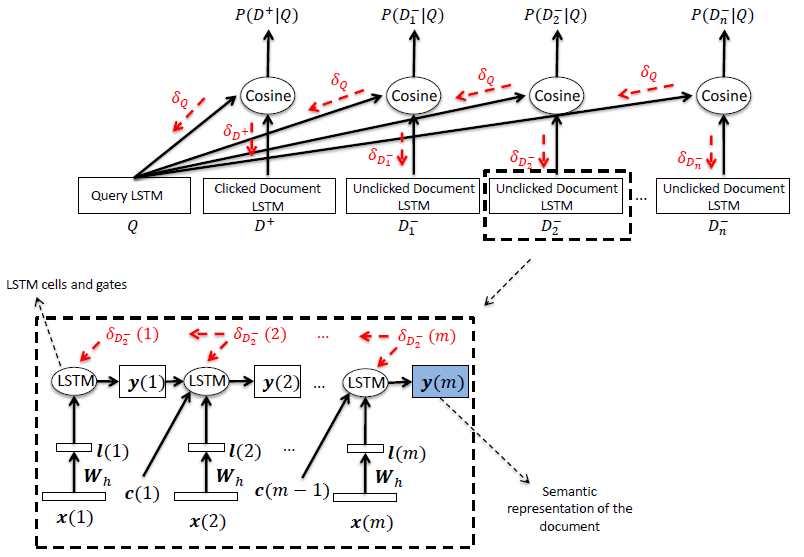
\includegraphics[width=0.8\linewidth]{figures/LSTM-DSSM.png}
  \caption{LSTM-DSSM模型结构}
  \label{fig:LSTM-DSSM}       % Give a unique label
\vspace{1em}
\end{figure}

DSSM及其衍生模型都是端到端的模型,虽然省去了算法工程师特征工程部分操作,但其效果不可控;而且DSSM都是若监督模型,需要大量的训练样本进行训练。DSSM模型论文中作者提到实际训练所使用的样本量超过一亿,而且论文中所使用的样本都是曝光置信度比较高的样本。这些限制因素极大地限制了DSSM的使用场景,往往只有少量大公司才可以使用。

因而,有研究学者关注直接利用深度学习建模匹配模型的方式,提取句子之间的各个级别的交互特征,这种方式更加直观,也更符合人类判断两个句子是否相似的过程。

MatchPyramid\cite{Pang2016TextMA}利用匹配矩阵建模两个句子的交互过程,如图~\ref{fig:MatchPyramid}。匹配矩阵中每个值都是2个句子中词两两计算得到的相似度。相似度可以使用词向量的余弦相似度或点积等进行刻画,而2个词在各自句子中的位置自然组成了一个二维坐标,开创性的构造出了单词级别相似性矩阵,即匹配矩阵。之后将匹配的问题建模为在这个匹配矩阵上进行图像识别的过程,这也是MatchPyramid的一大创新点。利用卷积和池化操作捕捉单词、短语、句子级别的交互信息,类似金字塔的层次结构,最终经过全连接得到句子之间的匹配程度。

\begin{figure}[!htbp]
\vspace{1em}
\centering
  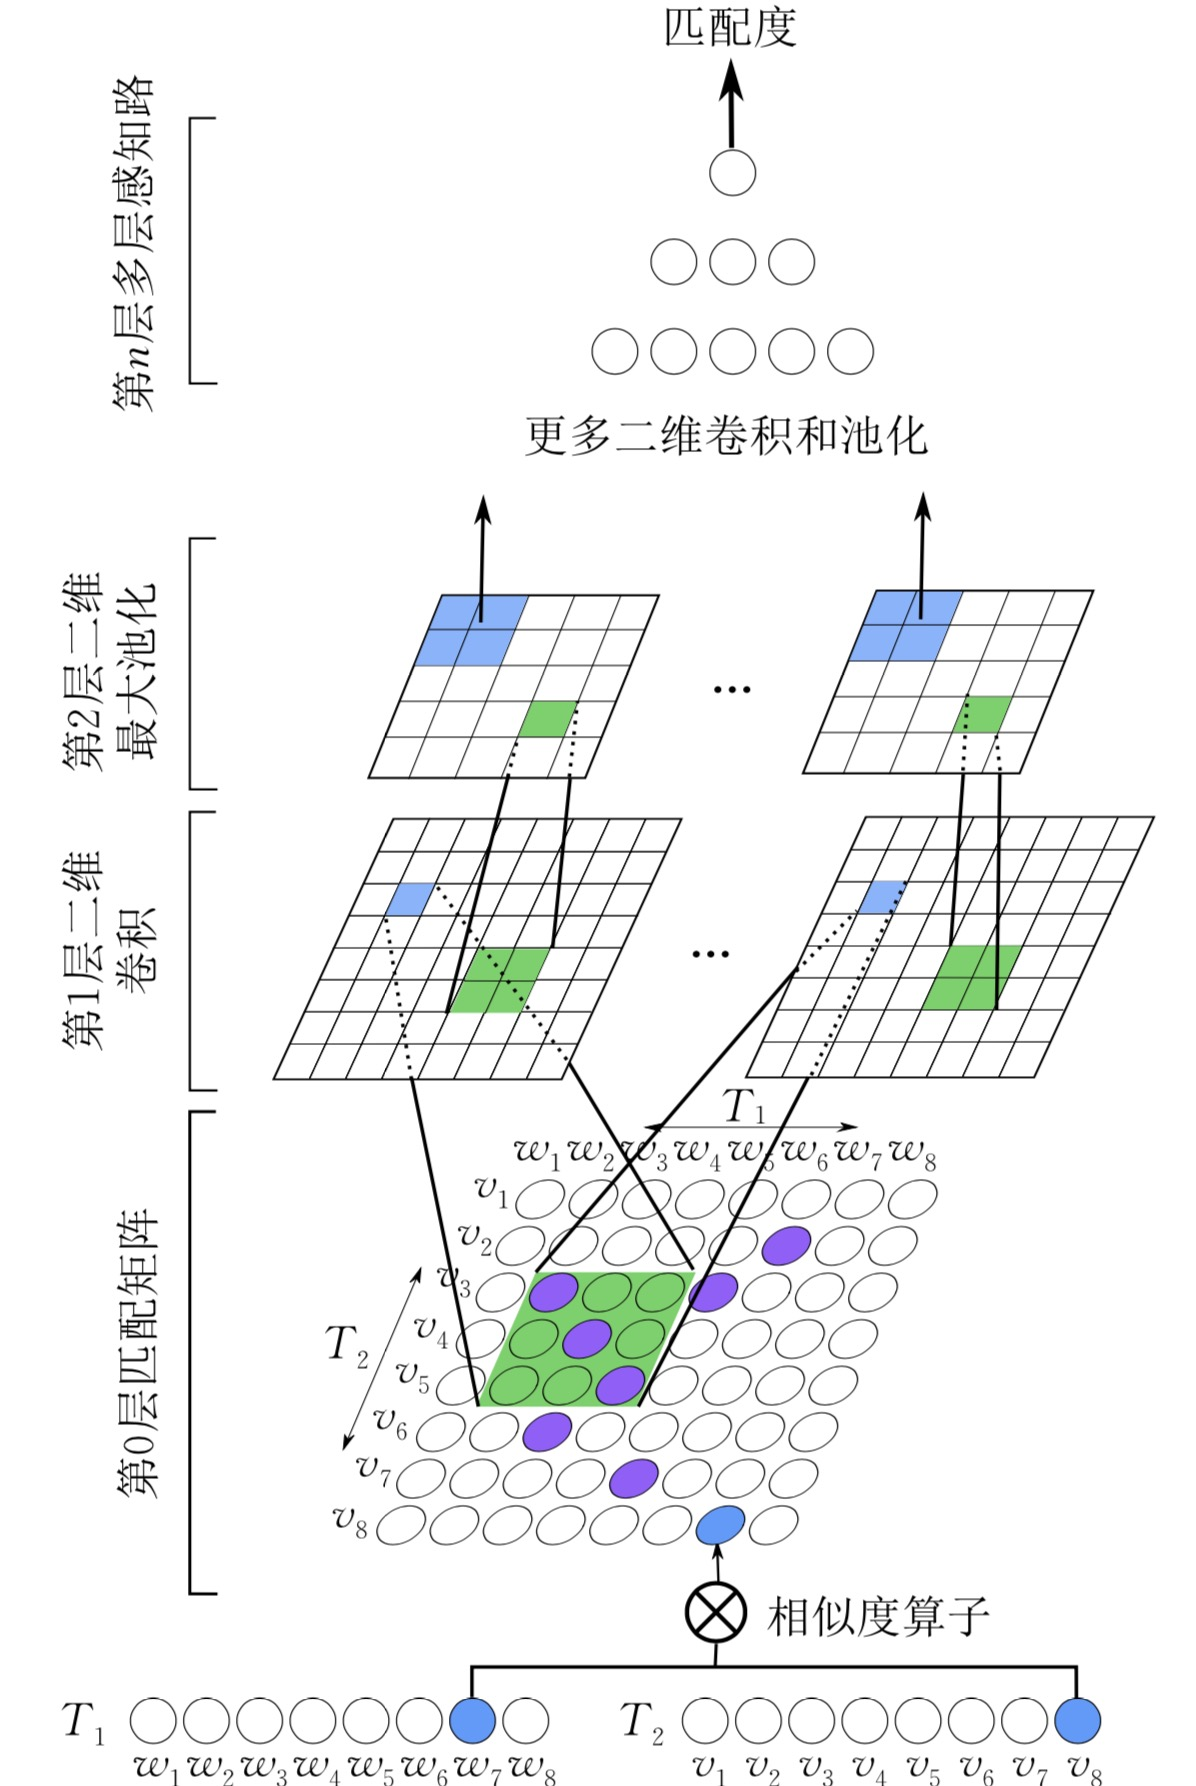
\includegraphics[width=0.45\textwidth]{figures/MatchPyramid.jpg}
  \caption{MatchPyramid模型}
  \label{fig:MatchPyramid}       % Give a unique label
\vspace{1em}
\end{figure}



但是,和CDSSM类似,利用分层结构的CNN建模文本匹配的过程,可能会失去上下文信息,使用序列结构的RNN优势更加显著。

有学者提出了MatchSRNN\cite{Wan2016MatchSRNNMT},MatchSRNN首先是用单词交互张量即匹配矩阵表示单词级别的交互信息,然后利用二维RNN\cite{Graves2007MultidimensionalRN}递归的整合局部交互信息,最后的匹配分数是由全局交互信息计算的。单词交互张量是表达一对文本中各个词向量之间交互信息的神经张量网络。普通一维RNN的当前状态 $\vec{h}_{t}$ 是由前一时刻状态 $\vec{h}_{t-1}$ 和当前输入 $\vec{x}_{t}$决定的,而在张量网络上运行的RNN则将其扩展到了二维空间,它当前位置状态由左方、上方、对角线方向上的前一位置 $\vec{h}_{i-1,j},\vec{h}_{i,j-1},\vec{h}_{i-1,j-1}$ 与当前位置上的输入 $\vec{s}_{ij}$ 的共同决定,RNN输入如~\eqref{spatial_rnn}~:
\begin{equation}
\label{spatial_rnn}
\vec{h}_{ij} = f(\vec{h}_{i-1,j},\vec{h}_{i,j-1},\vec{h}_{i-1,j-1},\vec{s}_{ij})
\end{equation}


MatchSRNN使用了RNN的变种门控循环单元\cite{Cho2014LearningPR}(Gated Recurrent Unit,GRU)GRU是LSTM的简化,只有更新门和重置门,重置门决定了如何将新的输入信息与前面的记忆相结合,更新门定义了前面记忆保存到当前时间步的量。GRU的计算方式:
\begin{equation}
\label{gru}
\begin{aligned}
r_t &= \sigma(W_r[h_{t-1},x_t])\\
z_t &= \sigma(W_z[h_{t-1},x_t])\\
\tilde{h}_t &= \text{tanh}(W_{\tilde{h}}[r_t \times h_{t-1},x_t]) \\
h_t &= (1-z_t)\times h_{t-1} + z_t\times\tilde{h}_t
\end{aligned}
\end{equation}

MatchSRNN用GRU遍历匹配矩阵,计算了每个门在三个方向上的值,如图\ref{fig:MatchSRNN},使用SoftmaxByRow对每一个维度进行线性变换,最后对二维GRU进行全连接层,非线性变换得到了最后的匹配程度。
\begin{figure}[!htbp]
\vspace{1em}
\centering
  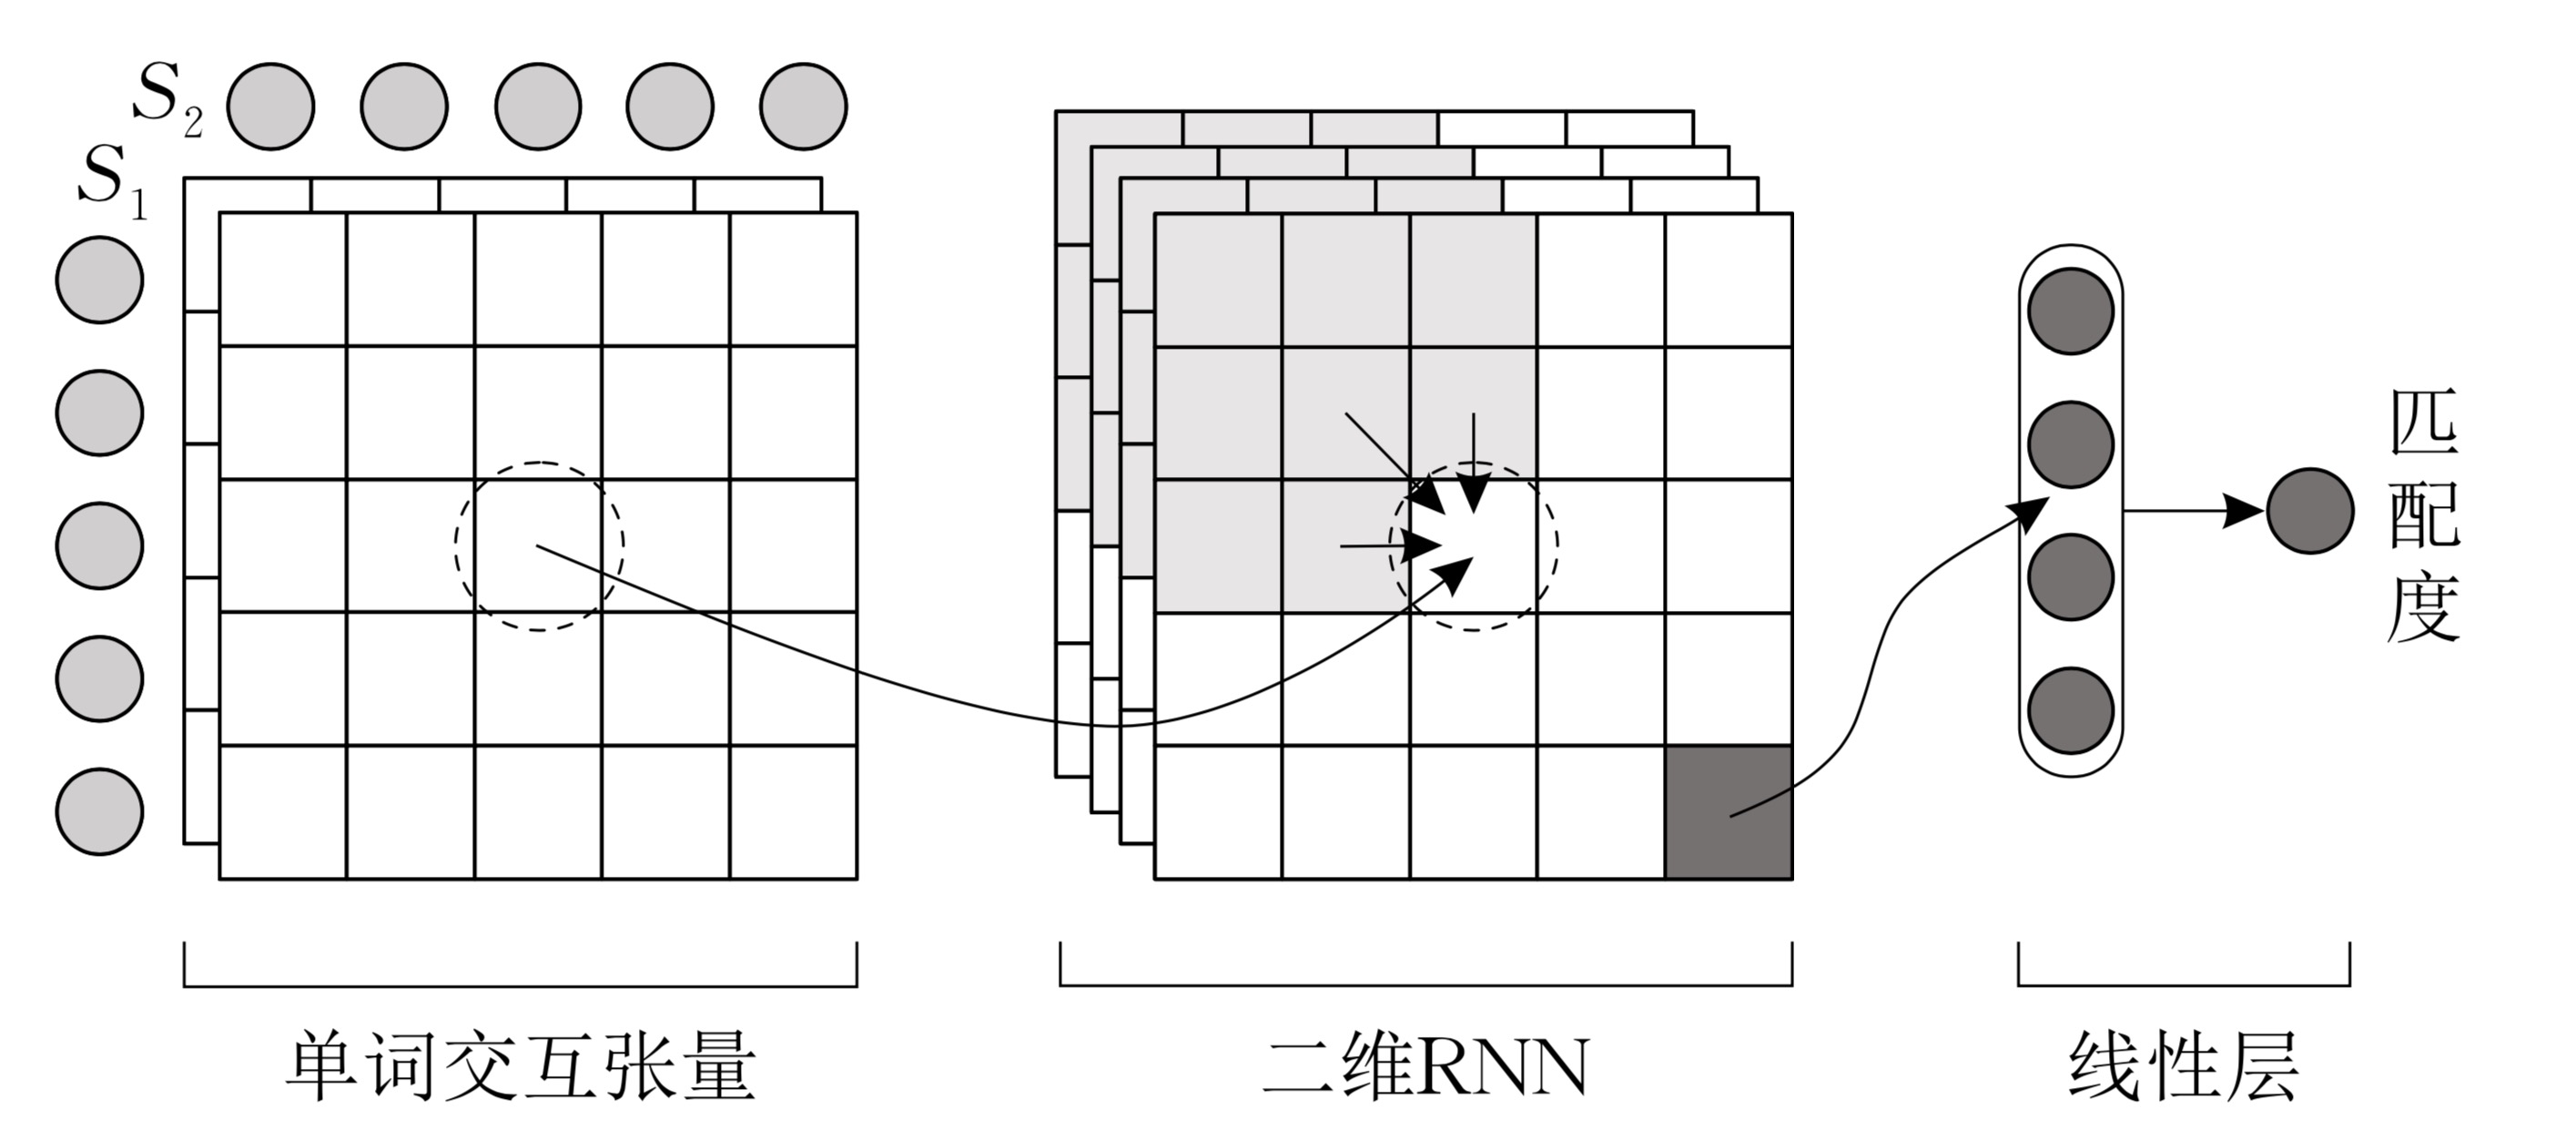
\includegraphics[width=0.9\linewidth]{figures/MatchSRNN.jpg}
  \caption{MatchSRNN模型}
  \label{fig:MatchSRNN}       % Give a unique label
\vspace{1em}
\end{figure}



\section{强化学习研究现状}
强化学习是机器学习中与监督学习、非监督学习并列的一个重要研究领域,它的本质是解决序列决策的问题,即自动进行决策,并且可以做连续决策\cite{Sutton1998ReinFORcementL}。和监督学习给定标注不同,强化学习给定的是一个奖励函数,主体(agent)以试错(trial-and-error)的机制与环境进行交互,最终目标是使主体在与环境交互中得到最大的累计奖励。这类算法有三个特征:闭环性,学习系统产生的行为会影响到后续的输出;无监督,学习对象只能通过学习去得这这些信息;延时性,行动(action)产生的结果,包括奖励(reward),需要很多个时间周期才能显现出来。强化学习中最基本的要素是主体和环境,除了这二者之外,还有四个要素策略、奖励信号、价值函数、对环境的建模(model)。其中:
\begin{itemize}
  \item 策略(Policy,$\pi$)定义了主体在给定时间内的行为方式,是从环境到这些状态下采取行动的映射,是强化学习主体的核心,可能是简单函数或查找表,也可能是随机的;

  \item 奖励信号(Reward signal,$R$)定义了强化学习问题的目标。在每个时间步骤,环境都会向主体发送一个奖励信号,主体唯一的目标是最大限度的提高长期得到的总奖励,因而奖励信号是改变策略的主要依据,它也是一个函数;

  \item 价值函数(Value function,$V$)定义了长远的回报。一个状态的价值是从该状态开始,这个主体在未来可以预期积累的总价值。奖励决定了状态的直接内在可取性,价值表明各个状态考虑到未来状态的长期可取性;

  \item 模型(Model,$M$)推断环境会如何表现,即给定一个状态和行为,模型会预测下一个状态和下一个奖励,模型用于规划,通过历史信息,考虑可能的未来情况来确定行为的方式。不过不是每个强化学习方法都需要模型,有的问题可以使用无模型方法解决。
\end{itemize}

\begin{figure}[!htbp]
\vspace{1em}
\centering
  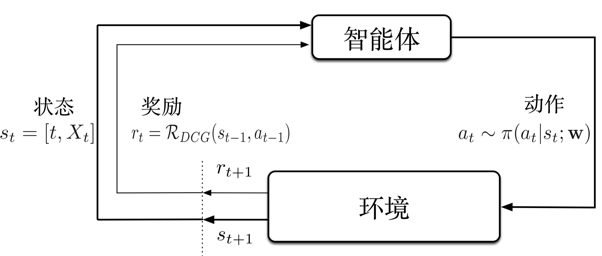
\includegraphics[width=0.8\linewidth]{figures/interaction.png}
  \caption{主体与环境的交互}
  \label{fig:LSTM-DSSM}       % Give a unique label
\vspace{1em}
\end{figure}

主体和环境的交互可以用图\ref{fig:interaction}表示。主体在当前状态$s_t$下根据策略π选择动作$a_t$,环境接收到该动作并转移到下一状态$s_{t+1}$,主体接收环境反馈回来的奖励选择下一步动作。强化学习不需要监督信号,主要算法包括Q学习(Q-learning),策略梯度(policy gradient)等等。

深度强化学习的主要思路是将神经网络用于抽取复杂高维数据中的信息,并将其映射到一个低维向量空间便于强化学习处理。
由于卷积神经网络在计算机视觉领域的统治地位,DeepMind团队在2013年尝试将卷积神经网络和强化学习结合,提出来深度Q网络(DeepQ Network,DQN)\cite{Mnih2013PlayingAW},并成功的将该方法用在了Atari视频游戏。这是深度强化学习首次在高维度的状态空间下起作用。

2015年,DeepMind团队进一步完善了DQN算法\cite{Mnih2015HumanlevelCT}。
DQN将深度卷积神经网络和Q学习结合到一起,并集成了经验回放技术(memory reply)和目标Q网络。
经验回放通过随机采样系统在探索环境时得到的状态数据对神经网络参数进行更新,打破了Q-学习算法采样数据之间的相关性。DQN在没有任何人类先验知识的情况下在Atari视频游戏表现出了等同人类玩家的水平纪念,是深度强化学习领域的重要工作。

2016年初,DeepMind团队发表了围棋AI:AlphaGo\cite{Silver2016MasteringTG}。AlphaGo 利用强化学习指导蒙特卡罗树搜索的过程,将深度强化学习的研究推向了新的高度。它通过策略网络学习不同位置的落子概率,利用价值网络学习棋局的胜率评估,通过策略和价值网络的结合减小了蒙特卡罗树搜索的搜索次数,提高了搜索效率。在在线对弈时,利用蒙特卡罗树搜索以及策略和价值网确定当前的落子位置。

\begin{figure}[!htbp]\centering
\vspace{1em}
  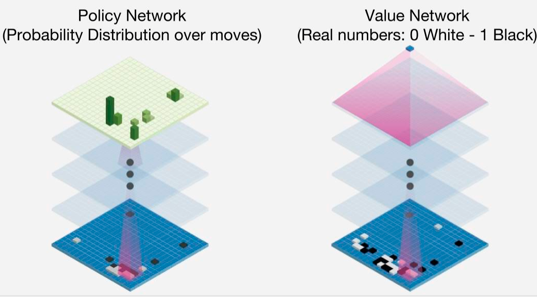
\includegraphics[width=0.8\linewidth]{AlphaGo.png}
  \caption{AlphaGo的策略网络和价值网络}  \label{fig:AlphaGo}       % Give a unique label
\vspace{1em}
\end{figure}

2017年初,AlphaGo Zero\cite{Silver2017MasteringTG}对AlphaGo进行了改进和升级。AlphaGo Zero 抛弃了 AlphaGo 复杂的特征输入,只需要将棋局图片作为数据即可;将策略网络和价值网络整合在一起,直接利用深度强化学习方法进行端到端的自我对弈学习。
相比于 AlphaGo,AlphaGo Zero 去除了棋手的落子网络,因此不需要任何先验知识;策略网络和价值网络的整合使得神经网络的复杂度降低,泛化性进一步增强,降低了硬件的资源需求,减少了训练时间。
\begin{figure}[!htbp]\centering
\vspace{1em}
  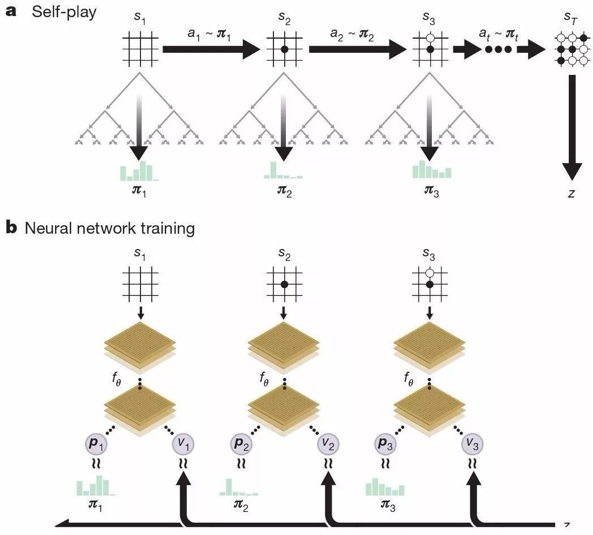
\includegraphics[width=0.5\linewidth]{AlphaGo_Zero.png}
  \caption{AlphaGo Zero 自我对弈训练过程} 
  \label{fig:AlphaGo_Zero}       % Give a unique label
  \vspace{1em}
\end{figure}
AlphaGo Zero的成功证明了在没有任何先验经验的情况下,深度强化学习在围棋领域仍然能取得巨大的成功;而在围棋下法上,AlphaGo Zero创造了更多的下棋方式,大大开拓了人类对围棋的认知。

\section{本章小结}

本章主要介绍了文本匹配和强化学习的相关工作与研究现状。

本章的第一小节主要介绍了基于深度学习的文本匹配算法。目前基于深度学习的文本匹配算法大都集中于利用神经网络理解输入句子的语义信息。最早利用深度学习解决文本匹配问题是DSSM。DSSM 利用词哈希以及词袋的方式得到句子的向量表示,并利用一个三层的全连接网络将句子的向量表示映射为一个低维向量表示。最后利用余弦相似度计算两个语义向量的距离,并利用 softmax 对得到的结果进行非线性变换,得到最后的概率分布。DSSM 通过词哈希降低了对且此算法的依赖,但是由于词袋模式的使用使其难以捕捉句子的上下文信息,而且全连接网络参数量极大,很难训练。为了解决 DSSM 模型问题,有人提出了CDSSM。相比于DSSM,CDSSM在词哈希的基础上引入了滑动窗口,通过滑动窗口解决了DSSM中上下文信息建模苦难的问题。同时 CDSSM 在表达网络中引入了卷积和池化操作,通过卷积建模上下文特征,利用池化发现全局特征,最后利用一个全连接层将结果映射到一个低维向量空间。但是由于卷积神经网络不是为序列化设置,因此对于长句子的上下文信息,CDSSN仍然难以捕捉。针对这个问题,有人提出将 LSTM 用于表达网络。DSSM及其后续的改进工作虽然有效的提高了文本匹配的效果,但是 DSSM 端到端的学习方式以及弱监督特征决定了它的利用场景十分有限。这种情况下有人提出了直接建模匹配模型的方法。MatchPyramid 利用两个句子之间词的相似度构造了一个匹配矩阵,将文本匹配过程视为对这个匹配矩阵的分类过程。 MatchPyramid 使用 CNN 建模了分类过程。和 MatchPyramid 类似, MatchSRNN 在匹配矩阵上使用了一个二维的 GRU 建模文本匹配的过程。

本章的第二小节主要介绍强化学习。强化学习是机器学习中的一个重要领域,最早用于机械控制领域,强调如何基于环境行动已获得最大收益。早期的增强学习方法包括策略梯度,值迭代等等,但是由于数据量过小,模型表达能力不强等等原因,强化学习的建模能力一直不强。近年来强化学习和深度学习的结合大大增加了强化学习的表达能力,使得强化学习近年来获得了长足的发展。DeepMind 提出了 DQN 并将其用于 Atari 游戏中,强化学习首次拥有了在高维状态空间下解决问题的能力。

16年初,DeepMind 团队提出了 AlphaGo 算法,该算法将强化学习和蒙特卡罗树搜索结合,通过策略网络和价值网络指导蒙特卡罗树搜索过程,大大提升了蒙特卡罗树搜索的速度。去年 DeepMind 进一步改进了 AlphaGo 算法,提出了 AlphaGo Zero。AlphaGo Zero 算法在没有任何人类先验知识的情况下在围棋领域取得了巨大的成功。

目前深度学习和强化学习的结合使得强化学习的表达能力大幅度上升,为学习传统文本匹配中复杂的规则和模式带来了可能。由于目前计算机理解人类语义十分困难,因此基于模式匹配的方式在短文本匹配场景中仍然拥有巨大的价值。本文会结合强化学习和文本匹配的特点,设计使用与文本匹配的强化学习算法。

\chapter{文本匹配问题的马尔可夫决策过程建模}
文本匹配的应用本章主要介绍了文本匹配问题的数学描述,强化学习的主要技术——马尔可夫决策过程以及面向文本匹配的算法设计。
\section{文本匹配描述}
为了更好地解决文本匹配问题,本节会利用数学符号形式化地定义文本匹配这个任务。

给定训练数据对,两个文本和一个标签: $(\mathbf{q}_1, \mathbf{d}_1, \mathbf{l}_1), (\mathbf{q}_2, \mathbf{d}_2, \mathbf{l}_2), \cdots, (\mathbf{q}_N, \mathbf{d}_N, \mathbf{l}_N)$,其中 $\mathbf{q}_i \in \mathbf{Q}$,$\mathbf{d}_i \in \mathbf{D}$为输入的一对文本,$\mathbf{l}_i \in \mathbf{L}$ 为标签,是0或1。在问答系统中,三者分别为问题、答案、答案能否回答问题;在问题复述中,三者分别为要判定是否同义的两个句子和是否同意义;在搜索引擎中,三者分别为查询、文档和是否相关。文本匹配的目标是自动学习训练数据上的匹配模型f,以便对于测试数据的每次输入,可以预测 $\mathbf{q}_i$ 和 $\mathbf{d}_i$ 的匹配程度 $\mathbf{r}_i$ ,可以设定一个阈值,若高于该阈值就认为为匹配,低于该阈值就认为不匹配。

在匹配的过程中,有一些关键步骤可以形式化的表述出来,以便

\section{马尔可夫决策过程}
强化学习研究的是如何根据环境的反馈,作出行动,从而最大化总收益。详细过程如下:在某一时刻 $t$ ,主体会处于状态 $s_t$,并从环境中得到观测 $o_t$,根据观测和行动利用策略 $\pi_\theta(a_t|o_t)$ 或者 $\pi_\theta(a_t|s_t)$作出行动 $a_t$,环境根据主体状态 $s_t$ 以及行动 $a_t$ 通过转移概率分布函数 $p(s_{t+1}| s_t, a_t)$ 得到状态 $s_{t+1}$,通过奖励函数 $r(s, a)$ 得到奖励 $r_t$,周而复始。而当环境是完全可观测的时候,它通常被形式化的描述为为马尔可夫决策过程(Markov Decision Process,MDP)几乎所有。强化学习中马尔可夫决策过程可以解决大部分问题\cite{Sutton1998ReinFORcementL},本小节会简要介绍马尔可夫决策过程及相关概念。

\subsection{马尔可夫相关概念}

在描述马尔可夫决策过程前,首先需要定义马尔可夫性质,一个状态有马尔可夫性质,当且仅当它满足式~\eqref{Markov}~,即在给定现在状态时,它与过去状态(即该过程的历史路径)是无关的。当前的状态已经包含了历史所有相关信息的状态,只要已知当前状态,可以丢弃所有历史信息,因为该状态已经足够预测未来。
\begin{equation}
\label{Markov}
\begin{aligned}
P[s_{t+1}|s_t]=P[s_{t+1}|s_1,\cdots,s_t]
\end{aligned}
\end{equation}

马尔科夫性描述的是每个状态的性质,马尔可夫链(或马尔可夫过程)$M=<\mathcal{S}, \mathcal{P}>$描述了一个状态序列,其中$\mathcal{S}$是状态空间,$s_t \in \mathcal{S}$是满足马尔可夫性质的随机状态,$\mathcal{P}$是一个状态转移概率矩阵,转移概率$p(s_{t+1}|s_t)$ 确定了在当前状态下转移到下一个状态的概率。令转移概率 $\mathcal{P}_{s, s'}=\mathbb{P}[S_{t+1}=s'|S_t=s]$,则这些概率组成了概率转移矩阵 $\mathcal{P}$。马尔科夫链具有马尔科夫性,即转移概率只与当前的状态有关。

马尔可夫决策过程是马尔可夫链在决策环境中的扩展 $M=<\mathcal{S}, \mathcal{A}, \mathcal{P}, \mathcal{R}, \gamma>$。其中:状态空间 $\mathcal{S}$ 与马尔科夫链类似;行动空间 $\mathcal{A}$ 即行动的集合;转移概率 $\mathcal{P}$ 不仅受到当前状态的影响,还受到行动 $a\in \mathcal{A}$ 的影响,定义为$\mathcal{P}_{s, s'}^{a}=\mathbb{P}[S_{t+1}=s'|s_t=s, A=a]$;$\mathcal{R}$ 为奖励函数,定义为$\mathcal{R}_{s}^{a}=\mathbb{E}[R_{t+1}|S_t=s, A_t=a]$,是一个 $\mathcal{S}\times A\to \mathbb{R}$ 的映射;$\gamma \in [0,1]$是衰减因子。

\begin{figure}[!htbp]\centering
\vspace{1em}
  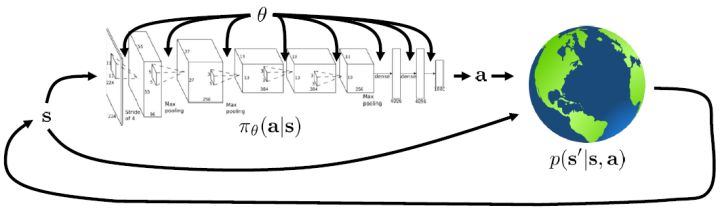
\includegraphics[width=0.9\linewidth]{figures/MDP.jpg}
  \caption{马尔可夫决策过程} 
  \label{fig:MDP}       % Give a unique label
  \vspace{1em}
\end{figure}


马尔可夫决策过程,按如下进行:主体初始状态$s_0$,然后按策略执行动作$a_0$,根据转移概率$\mathcal{P}_{s_0, s_1}^{a_0}$,跳转到下一个状态$s_1$,再执行动作$a_1$,转移到$s_2$,如图
\begin{figure}[!htbp]\centering
\vspace{1em}
  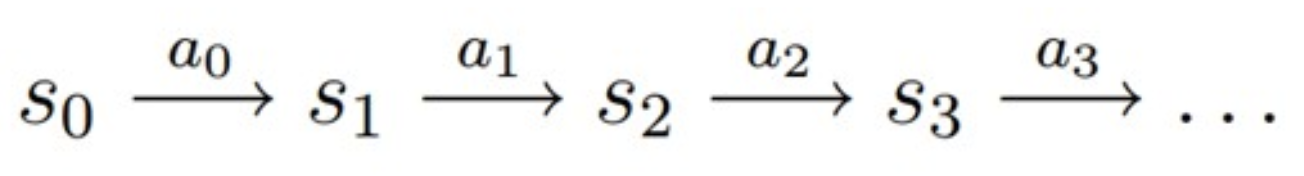
\includegraphics[width=0.9\linewidth]{figures/MDP_trans}
  \caption{MDP状态转移} 
  \label{fig:MDP}       % Give a unique label
  \vspace{1em}
\end{figure}

考虑一个有限长度的轨迹 $\tau=\{s_1,a_1,...s_t,a_t\}$,它产生的概率如式~\eqref{finite}~
\begin{equation}
\label{finite}
\begin{aligned}
p_\theta(\tau) = p(s_1)\prod_{t=1}^T \pi_\theta(a_t|s_t)p(s_{t+1}|s_t,a_t)
\end{aligned}
\end{equation}

初始状态 $s_1$ 往往是确定的。根据马尔科夫性,后面每个时刻的行动和状态都是由当前的行动确定的。我们希望优化式~\eqref{optimization}~以最大化总收益函数关于轨迹的期望。
\begin{equation}
\label{optimization}
\begin{aligned}
\theta^* = \arg\max_\theta E_{\tau\sim p_\theta(\tau)}[\sum_t r(s_t, a_t)]
\end{aligned}
\end{equation}


对于有限长度的轨迹,我们在求解 $\theta^*$ 时只需要关注马尔科夫链在一个时间点上的边际分布;对于无限长度的轨迹,根据马尔科夫性,有式~\eqref{MDP_finite}~:
\begin{equation}
\label{MDP_finite}
\begin{aligned}
\left[\begin{array}{l}\mathbf{s}_{t+k}\\\mathbf{a}_{t+k}\end{array}\right]=\mathcal{P}\left[\begin{array}{l}\mathbf{s}_{t+k-1}\\\mathbf{a}_{t+k-1}\end{array}\right]=...=\mathcal{P}^k\left[\begin{array}{l}\mathbf{s}_{t}\\\mathbf{a}_{t}\end{array}\right]
\end{aligned}
\end{equation}

对于无限长度的问题,当到达平稳分布时,我们可以对目标进行平均,如式~\eqref{infinite}~:
\begin{equation}
\label{infinite}
\begin{aligned}
\theta^*=\arg\max_\theta\frac{1}{T}\sum_{t=1}^T\mathbf{E}_{(\mathbf{s}_t,\mathbf{a}_t)\sim p_\theta(\mathbf{s}_t,\mathbf{a}_t)}r(\mathbf{s}_t,\mathbf{a}_t)\rightarrow \mathbf{E}_{(\mathbf{s},\mathbf{a})\sim p_\theta(\mathbf{s},\mathbf{a})}r(\mathbf{s},\mathbf{a})
\end{aligned}
\end{equation}

马尔可夫决策过程能够解决大部分强化学习问题,而一个完整的强化学习的训练过程,如图\ref{fig:RL_process}一般包含 3 个部分:

1. 生成样本。在模拟器中运行我们当前的策略并收集轨迹(trajectory)样本。轨迹的收集即主体和环境的交互过程:在 $t$ 时刻,我们从环境得到观测信息 $o_t$,在此观测信息下根据策略 $\pi_\theta(a_t|o_t)$ 得到当前的行动 $a_t$,根据系统的转移概率 $p(s_{t+1}|s_t, a_t)$ 得到下一个状态 $s_{t+1}$。在做出当前的行动之后,我们会得到收益 $r(s_t,a_t)$, 简记为 $r_t$ 。我们的目标就是最大化得到的总收益。

2. 收益估计。不同的算法在这一步的表现不尽相同。对于策略学习来说,就是策略评估;对于基于模型的增强学习算法,就是模型拟合。

3. 改进策略。根据上一步得到的结果改进策略,再执行第一步,循环往复。
\begin{figure}[!htbp]\centering
\vspace{1em}
  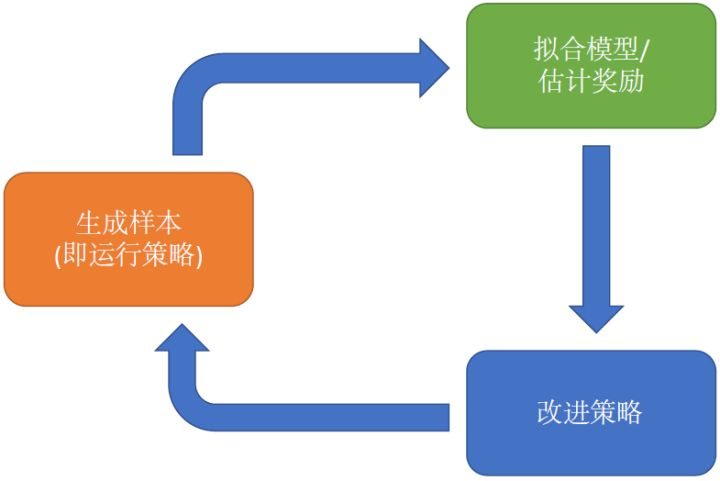
\includegraphics[width=0.6\linewidth]{figures/RL_process.jpg}
  \caption{强化学习算法一般步骤} 
  \label{fig:RL_process}       % Give a unique label
  \vspace{1em}
\end{figure}

\subsection{马尔可夫决策过程求解}
求解马尔可夫决策过程,除上述五元组外,还需要定义一些概念:
\begin{itemize}
\item 策略$\pi$:$\pi(a|s)=\mathbb[A_t=a|S_t=s]$,根据给定状态的行动分布。策略能够完全决定主体的行为。
\item 回报$G_t$:$G_t = R_{t+1} + \gamma R_{t+2} + ... = \sum_{k=0}^\infty \gamma^kR_{t+k+1}$ 从时间步$t$开始累积的经过衰减的总奖励,即奖励期望。
\item 价值函数$v(s)$:$v(s)=\mathbb{E}_{pi}[G_t|S_t=s]$ 从状态$s$开始,遵循策略$\pi$的预期回报,价值函数是一个状态在未来的价值,即回报的期望。
%\item 状态价值函数$v_{\pi}(s)$:$v_{\pi}(s)=\mathbb{E}_{\pi}[G_t|S_t=s]$ 根据状态$s$和策略$\pi$确定的状态价值。
%\item 行为价值函数$q_{\pi}(s,a)$:$q_{\pi}(s)=\mathbb{E}_{pi}[G_t|S_t=s,A_t=a]$ 从状态$s$开始,采取行动$a$,遵循策略$\pi$的预期回报
\end{itemize}
值函数可被分为两部分,立即奖励$R_{t+1}$和经过衰减的后继状态价值:
\begin{equation}\label{eq:Bellman}
\begin{aligned}
v(s) & = \mathbb{E}[G_t|S_t = s] \\
     & = \mathbb{E}[R_{t+1} + \gamma R_{t+2} + \gamma^2 R_{t+3}+...|S_t=s]\\
     & = \mathbb{E}[R_{t+1} + \gamma(R_{t+2} + \gamma R_{t+3}+...)|S_t=s]\\
     & = \mathbb{E}[R_{t+1} + \gamma G_{t+1}|S_t=s]\\
     & = \mathbb{E}[R_{t+1} + \gamma v(S_{t+1})|S_t=s]\\
\end{aligned}
\end{equation}

~\eqref{eq:Bellman}~被称为Bellman方程\cite{bellman1957markovian},它表明价值函数可以通过迭代计算得到,马尔可夫决策过程的目的就是通过迭代最大化$v(s)$。

通过Bellman方程,可以得到~\eqref{bellman2}~,通过迭代计算价值函数来优化策略,收敛到最优。
\begin{equation}\label{bellman2}
\begin{aligned}
v_{k+1}(s) &= \mathbb{E}[R_{t+1}+\gamma v_k(S_{t+1})|S_t=s]\\
		   &= \sum_a \pi(a|s) \sum_{s',r}p(s',r|s,a)[r+\gamma v_k(s')]	
\end{aligned}		   
\end{equation}

策略迭代一般分为策略评 估和策略改进。策略评估(Policy Evaluation):利用当前策略产生新样本;策略改进(Policy Improvement):使用新样本更新当前策略,最终收敛到最优。在策略评估时需要知道环境的状态转移概率,因此策略迭代需要依赖模型。

\begin{algorithm}[H]
    \small
    \caption{policy iteration}\label{alg:policy_iteration}
    \begin{algorithmic}
        \STATE Step 1. Initialization
        	\STATE $V(s) \in \mathbb{R}$ and $\pi(s) \in \mathcal{A}(s)$ arbitrarily FOR all $s \in \mathcal{S}$
        \STATE Step 2. Policy Evaluation
        \REPEAT
        \STATE $\Delta \leftarrow 0$
        \FOR {each $s \in \mathcal{S}$}
        \STATE $v \leftarrow V(s)$
        \STATE $V(s)\leftarrow \sum_{s', r} p(s', r|s, \pi(s))[r + \gamma V(s')]$
        \STATE $\Delta \leftarrow \max(\Delta, |v-V(s)|$
        \ENDFOR

        \UNTIL{$\Delta < \theta$}

        \STATE Step 3. Policy Improvement
        \STATE policy-stable $\leftarrow  true$
        \FOR {each $s \in \mathcal{S}$}
        \STATE $a \leftarrow \pi(s)$
        \STATE $\pi(s) \leftarrow \arg\max_a\sum_{s', r}p(s', r|s, \pi(s))[r + \gamma V(s')]$
        \STATE If $a \neq \pi(s)$ then policy-stable $\leftarrow  false$
        \ENDFOR
        \STATE If policy-stable, then stop and return V and $\pi$; else go to 2
    \end{algorithmic}
\end{algorithm}

策略迭代算法每次都要进行策略评估和改进,大大增加了算法的训练时间,由于对文本匹配问题对策略的改进和对值函数的改进是一致的,所以可以将策略改进视为对值函数的改进。

通过Bellman方程,我们可以得到:

\begin{equation}\label{bellman_val}
	\begin{aligned}
		v_*(s) &= \mathbb{E}[R_{t+1}+\gamma v_*(S_{t+1})|S_t=s,A_t=a]
			   &= \max_a \sum_{s',r}p(s', r|s, a)[r+\gamma v_k(s')]
	\end{aligned}
\end{equation}

从\eqref{bellman_val}可以发现,我们可以通过Bellman最优模型来更新值函数收敛,最后收敛可以得到当前策略的最优值$v_*$。

\begin{algorithm}[!htbp]
    \small
    \caption{value iteration}\label{alg:value_iteration}
    \begin{algorithmic}
        \STATE Initialization array $V$ arbitrarily
        \REPEAT
        \STATE $\Delta \leftarrow 0$
        \FOR {each $s \in \mathcal{S}$}
        \STATE $v \leftarrow V(s)$
        \STATE $V(s)\leftarrow \max_a\sum_{s', r} p(s', r|s, a)[r + \gamma V(s')]$
        \STATE $\Delta \leftarrow max(\Delta, |v-V(s)|$
        \ENDFOR
        \UNTIL {$\Delta < \theta$}

        \STATE Output a deterministic policy, $\pi$ such that
        \STATE $\pi(s) = \arg\max_a\sum_{s', r} p(s', r|s, a)[r + \gamma V(s')]$
    \end{algorithmic}
\end{algorithm}



相比于算法~\ref{alg:policy_iteration}~,值迭代算法~\ref{alg:value_iteration}~避免了策略评估部分的计算量,降低了算法的运行时间,有效地提高了算法的运行效率。

我们发现无论是算法 \ref{alg:policy_iteration} 还是 \ref{alg:value_iteration},每次都是选择概率或者是值最高的行为,这种策略被称为利用(exploitaion)。与之对应的,如果我们每次都根据概率或者值的分布进行采样(sampling),根据采样的结果采取行动,这种策略被称为探索(exploration)。探索的优势在于当信息匮乏时,可以取得较好的效果;利用的优势在于效率很高,但只有在信息足够充足的情况下才会有效。

探索和利用各有优势,将二者结合的算法被称为$\epsilon$-贪心算法。我们在每次选择行动的时候,都以$\epsilon$的概率进行探索,以$1-\epsilon$的概率进行利用。可以通过 $\epsilon$ 的调整在算法的不同阶段达到不同的效果。


\section{面向文本匹配的马尔可夫决策过程建模}
\label{sec:TM_MDP}
本节将强化学习建模为一个马尔可夫决策过程。

在\ref{sec:text_matching} 节,中我们介绍了MatchSRNN\cite{Wan2016MatchSRNNMT} 算法。MatchSRNN 使用匹配矩阵中提取句子间的交互信息,利用二维 GRU 提取单个句子和句子之间的序列信息。 在二维 GRU计算完成后,通过二维 GRU 的状态,我们可以回溯出一条路径。
图\ref{fig:LD_dis}表示了对 $Q$=How to get rid of memory stick error of my
sony cyber shot?, $D$=You might want to try to FORmat the memory
stick but what is the error message you are receiving. 得到的匹配矩阵进行回溯得到的路径。

\begin{figure}[!htbp]\centering
\vspace{1em}
  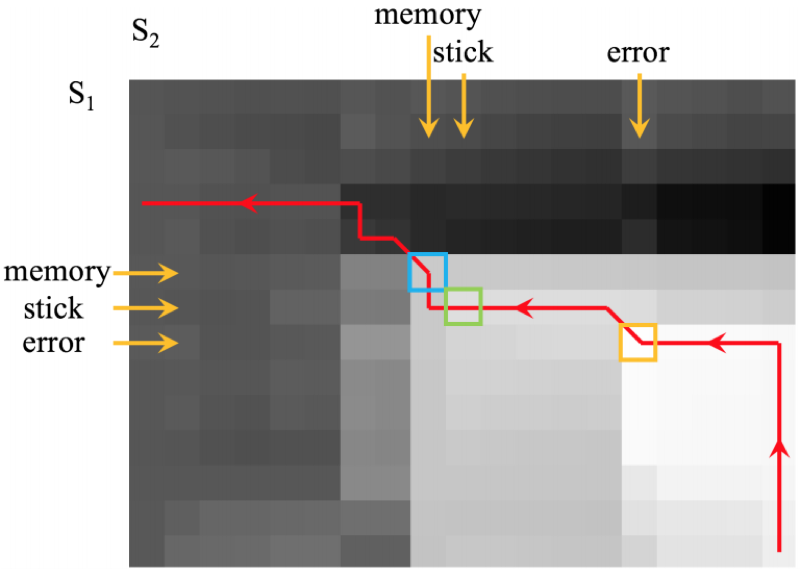
\includegraphics[width=0.6\linewidth]{figures/LD_dis}
  \caption{MatchSRNN的回溯路径} 
  \label{fig:LD_dis}       % Give a unique label
  \vspace{1em}
\end{figure}

既然MatchSRNN通过回溯可以得到一条路径,那么一个直接的想法就是不通过二维GRU的方式直接获得一条路径,利用这条路径判断这两个句子是否匹配。

\begin{figure}[!htbp]\centering
\vspace{1em}
  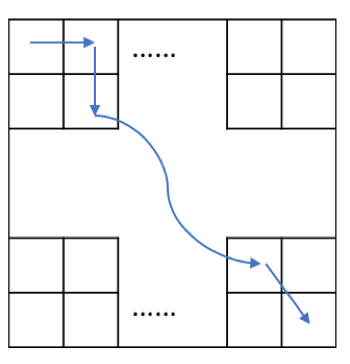
\includegraphics[width=0.5\linewidth]{figures/match_MDP}
  \caption{文本匹配路经计算过程} 
  \label{fig:match_MDP}       % Give a unique label
  \vspace{1em}
\end{figure}

和MatchPyramid以及MatchSRNN类似,我们同样会使用匹配矩阵的概念。从匹配矩阵左上角出发,根据当前位置,确定行动方向,直到走到右下角为止

\chapter{基于价值迭代的文本匹配算法实现}


%\section{评价指标}
%本节介绍用于文本匹配算法的评价指标。在本文中,文本匹配可被看作一个分类问题,判断一个二分类预测模型优劣的评价指标主要有:精确率(Precision),召回率(Recall),F值(F-score),准确率(Accuracy,ACC),受试者工作特征曲线(Receiver Operating Characteristic,ROC),AUC(Area Under Curve of ROC)。
%本文使用的是准确率,F1和AUC这三个指标。
%
%\begin{figure}[!htbp]
%\vspace{1em}
%\centering
%  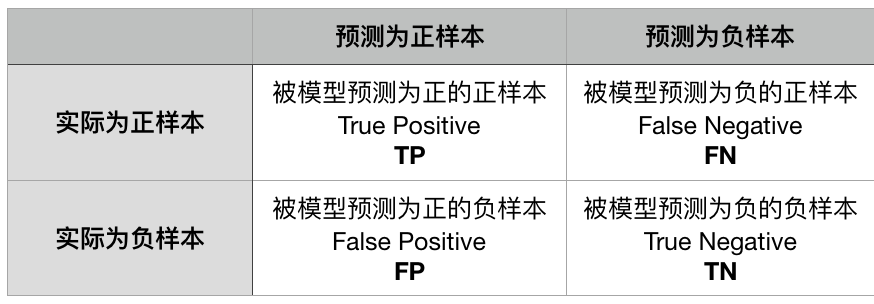
\includegraphics[width=0.9\linewidth]{figures/matrix}
%  \caption{混淆矩阵}
%  \label{fig:Con_matrix}       % Give a unique label
%\vspace{1em}
%\end{figure}
%
%图\ref{fig:Con_matrix}是混淆矩阵(Confusion Matrix)。本节出现的所有指标都是以该矩阵为依据。
%
%准确率$\text{ACC}$是计算样本被正确预测的次数占总样本的比例,如式~\eqref{acc_eq}~。准确率越高,算法在该指标上表现越好,当准确率为1时,该评价指标达到最优值。
%\begin{equation}
%\label{acc_eq}
%\begin{aligned}
%\text{ACC}=\frac{\text{TP}+\text{TN}}{\text{TP}+\text{FP}+\text{TN}+\text{FN}}
%\end{aligned}
%\end{equation}
%
%精确率是被模型预测为正的样本中,实际为正样本的比例,如式~\eqref{precision_eq}~,召回率是实际为正的样本中,正确预测为正样本的比例,如式~\eqref{recall_eq}~。
%\begin{equation}
%\label{precision_eq}
%\begin{aligned}
%\text{P}=\frac{\text{TP}}{\text{TP}+\text{FP}}
%\end{aligned}
%\end{equation}
%\begin{equation}
%\label{recall_eq}
%\begin{aligned}
%\text{R}=\frac{\text{TP}}{\text{TP}+\text{FP}}
%\end{aligned}
%\end{equation}
%
%$\text{F}_1$是精确率和召回率的调和平均数,相当于精确率和召回率的综合评价指标,如式~\eqref{f1_eq}~。$\text{F}_1$越大,算法在该指标上表现越好,当$\text{F}_1$为1时,该评价指标达到最优。
%\begin{equation}
%\label{f1_eq}
%\begin{aligned}
%\text{F}_1 &= \frac{2}{\frac{1}{P}+\frac{1}{R}} \\
%\text{F}_1 &= \frac{2*P*R}{P+R}
%\end{aligned}
%\end{equation}
%
%AUC就是ROC曲线和坐标轴相交部分覆盖的面积大小,ROC曲线由两个变量真正样本率TPR(True Positive Rate)和假正样本率FPR(False Positive Rate)绘制,其中TPR和FPR如式~\eqref{tpr_fpr}~,分别反映了正样本和负样本的分类准确率,AUC越大,算法在该指标上表现越好,当AUC为1时,该评价指标达到最优。
%\begin{equation}
%\label{tpr_fpr}
%\begin{aligned}
%\text{TPR} &= \frac{TP}{TP+FN} \\
%\text{FPR} &= \frac{FP}{FP+TN}
%\end{aligned}
%\end{equation}
%






\chapter{基于蒙特卡洛树搜索的文本匹配建模及实现}

很多和计算机专业背景相关的同学都会使用到代码环境,使用~\verb|\verb|~指令或者是~\verb|verbatim|~环境固然是一种选择,但是比不上专门的~lstlisting~环境这么专业。

\begin{lstlisting}
int main(int argc, char ** argv) {
    printf("Hello world!\n");
    return 0;
}
\end{lstlisting}

\section{普通表格的绘制方法}

表格应具有三线表格式,其标准格式如表 \ref{tab:table1} 所示。
\begin{table}[htbp]
\caption{符合本科生毕业论文绘图规范的表格}\label{tab:table1}
\vspace{0.5em}\centering\wuhao
\begin{tabular}{ccccc}
\toprule[1.5pt]
$D$(in) & $P_u$(lbs) & $u_u$(in) & $\beta$ & $G_f$(psi.in)\\
\midrule[1pt]
 5 & 269.8 & 0.000674 & 1.79 & 0.04089\\
10 & 421.0 & 0.001035 & 3.59 & 0.04089\\
20 & 640.2 & 0.001565 & 7.18 & 0.04089\\
 5 & 269.8 & 0.000674 & 1.79 & 0.04089\\
10 & 421.0 & 0.001035 & 3.59 & 0.04089\\
20 & 640.2 & 0.001565 & 7.18 & 0.04089\\
 5 & 269.8 & 0.000674 & 1.79 & 0.04089\\
10 & 421.0 & 0.001035 & 3.59 & 0.04089\\
20 & 640.2 & 0.001565 & 7.18 & 0.04089\\
 5 & 269.8 & 0.000674 & 1.79 & 0.04089\\
10 & 421.0 & 0.001035 & 3.59 & 0.04089\\
20 & 640.2 & 0.001565 & 7.18 & 0.04089\\
\bottomrule[1.5pt]
\end{tabular}
\vspace{\baselineskip}
\end{table}

%%%%%%% 结论 %%%%%%%

\addcontentsline{toc}{chapter}{结\quad 论} %添加到目录中

\chapter*{结\quad 论}

得出结论,楼主傻逼。
